\documentclass[a4paper,11pt,dvipdfmx]{jsarticle}


% 数式
\usepackage{amsmath,amsfonts}
\usepackage{bm}

% 画像
\usepackage[dvipdfmx]{graphicx}

% 図形
\usepackage{tikz}
\usetikzlibrary{shapes.geometric}
\usetikzlibrary {shapes.misc}
\usepackage{tikz-imagelabels}

% ソースコード
\usepackage{listings,jlisting,color}
\lstset{
basicstyle={\ttfamily},
identifierstyle={\small},
commentstyle={\smallitshape},
keywordstyle={\small\bfseries},
ndkeywordstyle={\small},
stringstyle={\small\ttfamily},
frame={tb},
breaklines=true,
columns=[l]{fullflexible},
numbers=left,
xrightmargin=0zw,
xleftmargin=3zw,
numberstyle={\scriptsize},
stepnumber=1,
numbersep=1zw,
lineskip=-0.5ex
}
\renewcommand{\lstlistingname}{ソースコード}


\begin{document}

\title{画像処理 課題1 トーンマッピング}
\author{21T2166D 渡辺大樹}
\date{2023/05/25}
\maketitle

\section{課題の目的・意図}
本課題では、ヒストグラムの幅(画像の輝度値の範囲)を広げる線形濃度変換と
逆光時などの明るさにばらつきが出た画像のヒストグラムの局所的、急激な変化の山を改善するヒストグラム平坦化を
用いて、コントラストの強調された、また明るさのばらつきが少ない画像を得ることを目的とし行う。

\section{処理内容}
以下では線形濃度変換とヒストグラム平坦化の二つの処理で実際に行っていることを説明していく。
\subsection{線形濃度変換}
線形濃度変換では低コントラスト、言い換えれば露出度が適切ではない画像の輝度値を解析し、その分布範囲を線形関数
を用いて広くすることで、色差の大きい画像を生成する。すなわち図\ref{hist_1}のような変換を行う。
\begin{figure}[htbp]
    \centering
    \begin{minipage}{0.4\hsize}
        \centering
        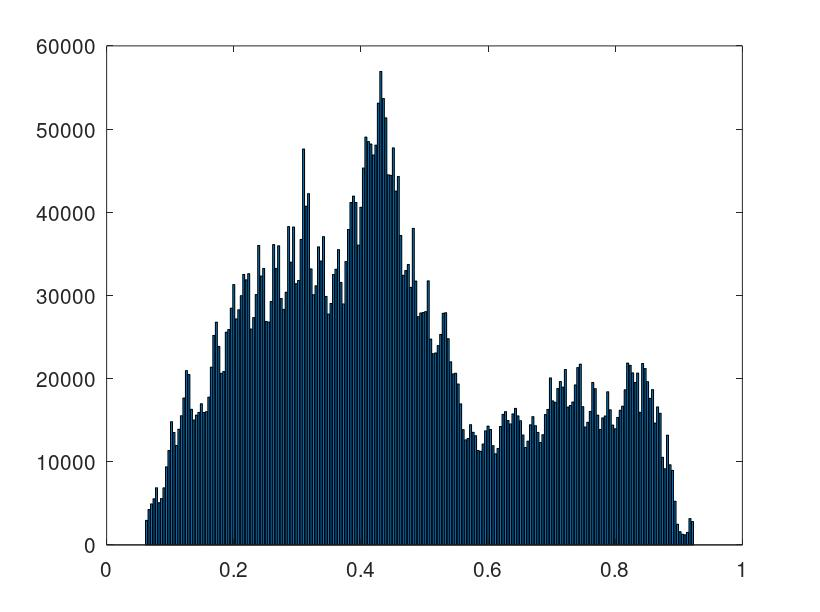
\includegraphics[width=50mm]{./img/linear_ex.jpg}
    \end{minipage}
    \begin{minipage}{0.1\hsize}
        \centering
        \begin{math}
                \overset{f(x)=ax+b}{\to}
        \end{math}
    \end{minipage}
    \begin{minipage}{0.4\hsize}
        \centering
        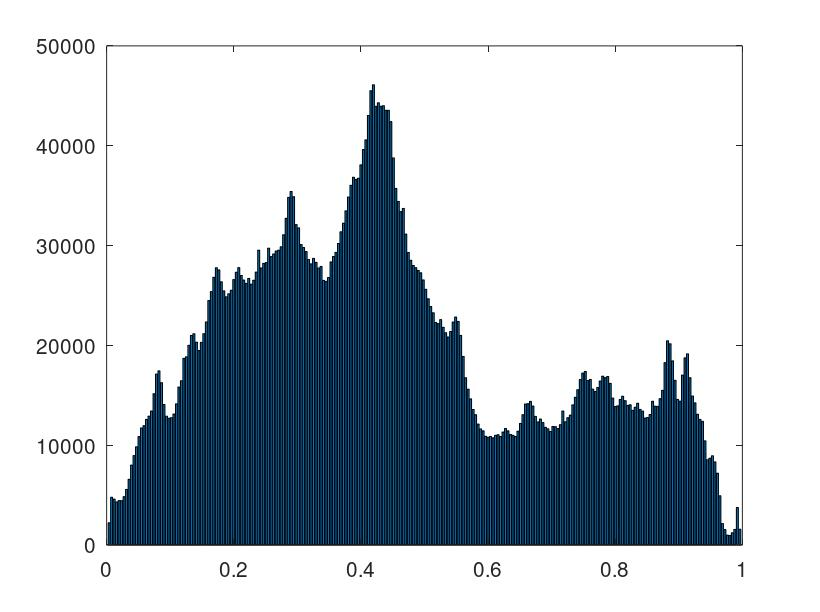
\includegraphics[width=50mm]{./img/linear_ex1.jpg}
    \end{minipage}
    \caption{線形濃度変換によるヒストグラムの変化例}
    \label{hist_1}
\end{figure}

そのためには処理前の画像から得られた輝度値から、その輝度値の範囲を確認。この変換前の輝度値の範囲を$x_1,x_2(x_1<x_2)$とすると、
これを輝度値の最大、最小値まで拡大するような線形関数を、この画像の輝度値全体に適応する必要がある。

入力画像の輝度値の範囲を$x_1,x_2$とし、出力画像の輝度値の範囲を$y_1,y_2$とする。

$y=ax+b$の形の線形関数を用いて変形を行うとき(この変形はアフィン変換という)定数である$a,b$は連立方程式

\begin{equation}
    \left \{ \,
    \begin{aligned}
        y_1 &= ax_1 + b \\
        y_2 &= ax_2 + b
    \end{aligned}
    \right .
\end{equation}
を解くことで求まる。これは$a,b$の係数行列と$(a,b)$の積であると考えれば

\begin{equation}
    \begin{pmatrix}
        y_1 \\ y_2
    \end{pmatrix}
    =
    \begin{pmatrix}
        x_1 & 1 \\
        x_2 & 1
    \end{pmatrix}
    \begin{pmatrix}
        a \\ b
    \end{pmatrix}
\end{equation}
となる。これは逆行列を用いて解くことができて、

\begin{equation}
    \frac{1}{x_1-x_2}
    \begin{pmatrix}
        y_1 - y_2 \\ -x_2y_1 + x_1y_2
    \end{pmatrix}
    =
    \begin{pmatrix}
        a \\ b
    \end{pmatrix}
\end{equation}
としてしまえば、

\begin{equation}
    \left \{ \,
    \begin{aligned}
        a &= \frac{y_1-y_2}{x_1-x_2} \\
        b &= \frac{-x_2y_1+x_1y_2}{x_1-x_2}
    \end{aligned}
    \right .
\end{equation}
と求まる。

これにより求まった式(4)の係数を利用するのが線形濃度変換の計算方法となる。

このヒストグラムの濃度変換はほかにも、
いくつかの区分の一次式、多項式を組み合わせたもの(スプライン関数)や$tan$関数などを用いることもある。

\subsection{ヒストグラム平坦化}
続いて、逆光時など明るさにばらつきがある画像を補正する処理、ヒストグラム平坦化について説明していく。

逆光などで明るさのばらつく画像は図\ref{hist_2}のようなヒストグラムになっている。
\begin{figure}[htbp]
    \centering
    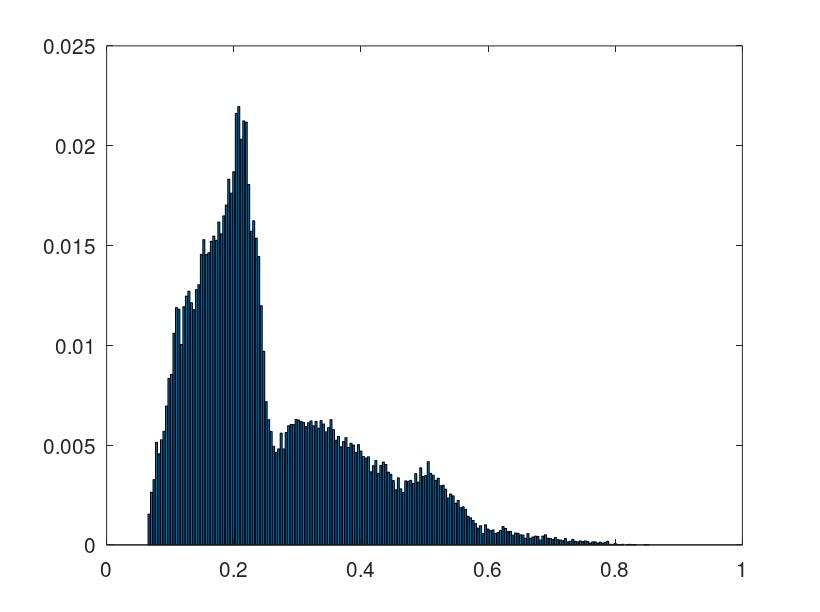
\includegraphics[width=80mm]{./img/flatten_ex.jpg}
    \caption{明るさにばらつきのある画像のヒストグラム}
    \label{hist_2}
\end{figure}

このようなヒストグラムに対して、ヒストグラムの山を広げるような処理をするのがヒストグラム平坦化である。

ヒストグラムの山を広げるという処理は線形濃度変換のようなシンプルなマッピング関数では実装が難しい。
そのため、ヒストグラム個別にマッピング関数を生成する必要がある。

このマッピング関数$f(x)$を求めるのは、複雑ではない。ヒストグラムの勾配が大きいところほど大きな山ができていることを
考えれば、このヒストグラム関数$h(x)$を単に積分してしまえばよい。
すなわち式にして表すと適当な0以上の係数$s$を用いて、式(5)のようになる。
\begin{equation}
    f(x) = s \int h(x)dx
\end{equation}

ただしヒストグラム関数が離散値であるので
\begin{equation}
    f(x) = \sum_{i=i}^{x}h(i)
\end{equation}
とすることで、入力画像毎にマッピング関数を決めることができる。

実際にこの処理を画像に施すと図\ref{hist_3}のようなヒストグラムの変換を行うことができる。

\begin{figure}[htbp]
    \centering
    \begin{tabular}{ccccc}
    \begin{minipage}[l]{0.2\hsize}
        \centering
        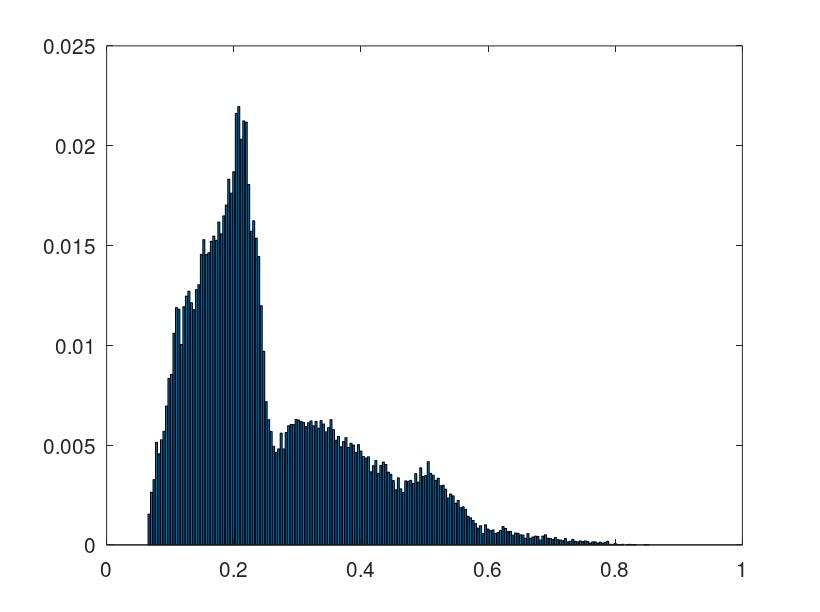
\includegraphics[width=40mm]{./img/flatten_ex.jpg}
    \end{minipage}&
    \begin{minipage}[c]{0.2\hsize}
        \centering
        \begin{math}
                \overset{f(x) = \sum_{i=i}^{x}h(i)}{\to}
        \end{math}
    \end{minipage}&
    \begin{minipage}[c]{0.21\hsize}
        \centering
        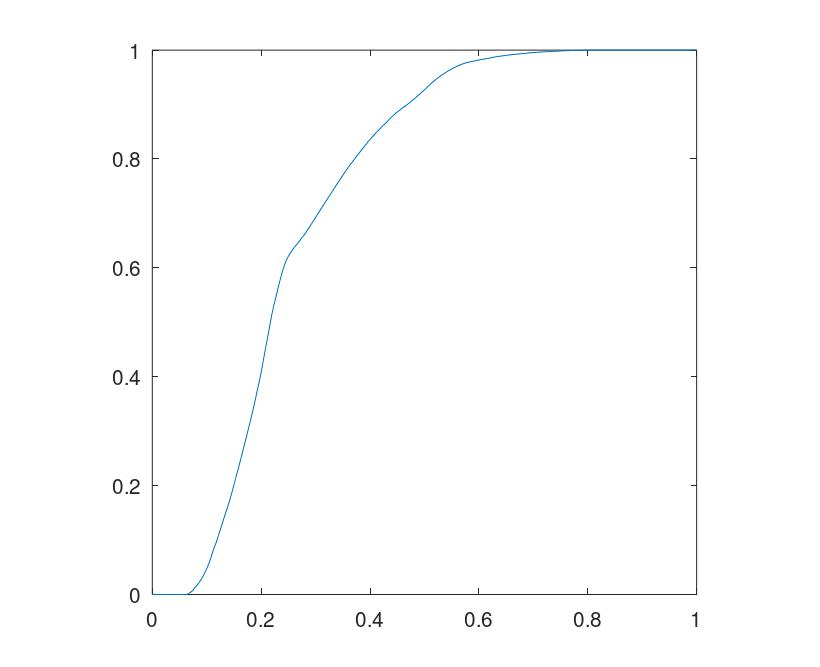
\includegraphics[width=30mm]{./img/flatten_func_ex.jpg}
    \end{minipage}&
    \begin{minipage}{0.12\hsize}
        \centering
        \begin{math}
                \overset{h'(x)=f(x)h(x)}{\to}
        \end{math}
    \end{minipage}&
    \begin{minipage}[c]{0.2\hsize}
        \centering
        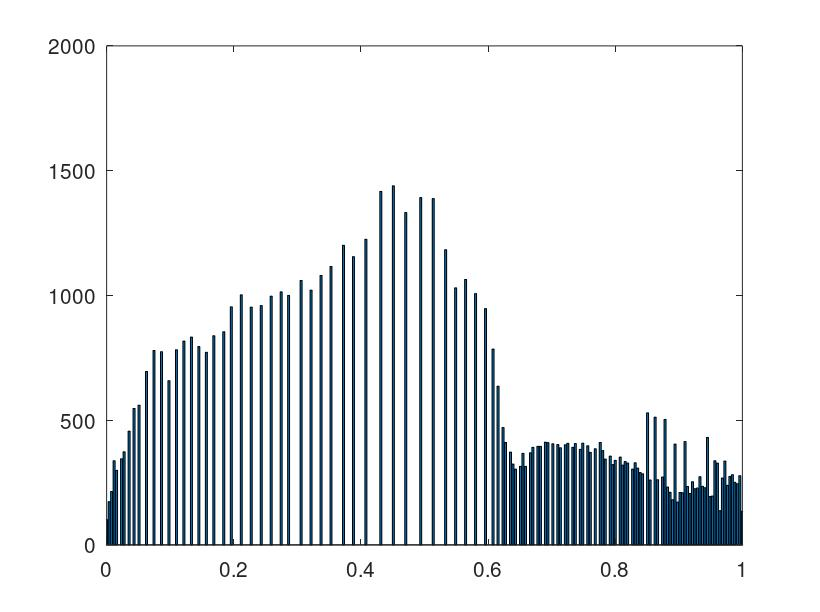
\includegraphics[width=40mm]{./img/flatten_ex2.jpg}
    \end{minipage}
    \end{tabular}
    \caption{ヒストグラム平坦化によるヒストグラムの変化例}
    \label{hist_3}
\end{figure}

これがヒストグラム平坦化の処理内容となる。

\section{演習}
では実際に、画像に対してヒストグラムの線形濃度変換とヒストグラム平坦化の処理を行う。

\subsection{線形濃度変換}
まず、線形濃度変換から行う。

図\ref{Morita}のような画像を用意した。これは上田市駅近くにある町中華モリタである。
\begin{figure}[htbp]
    \centering
    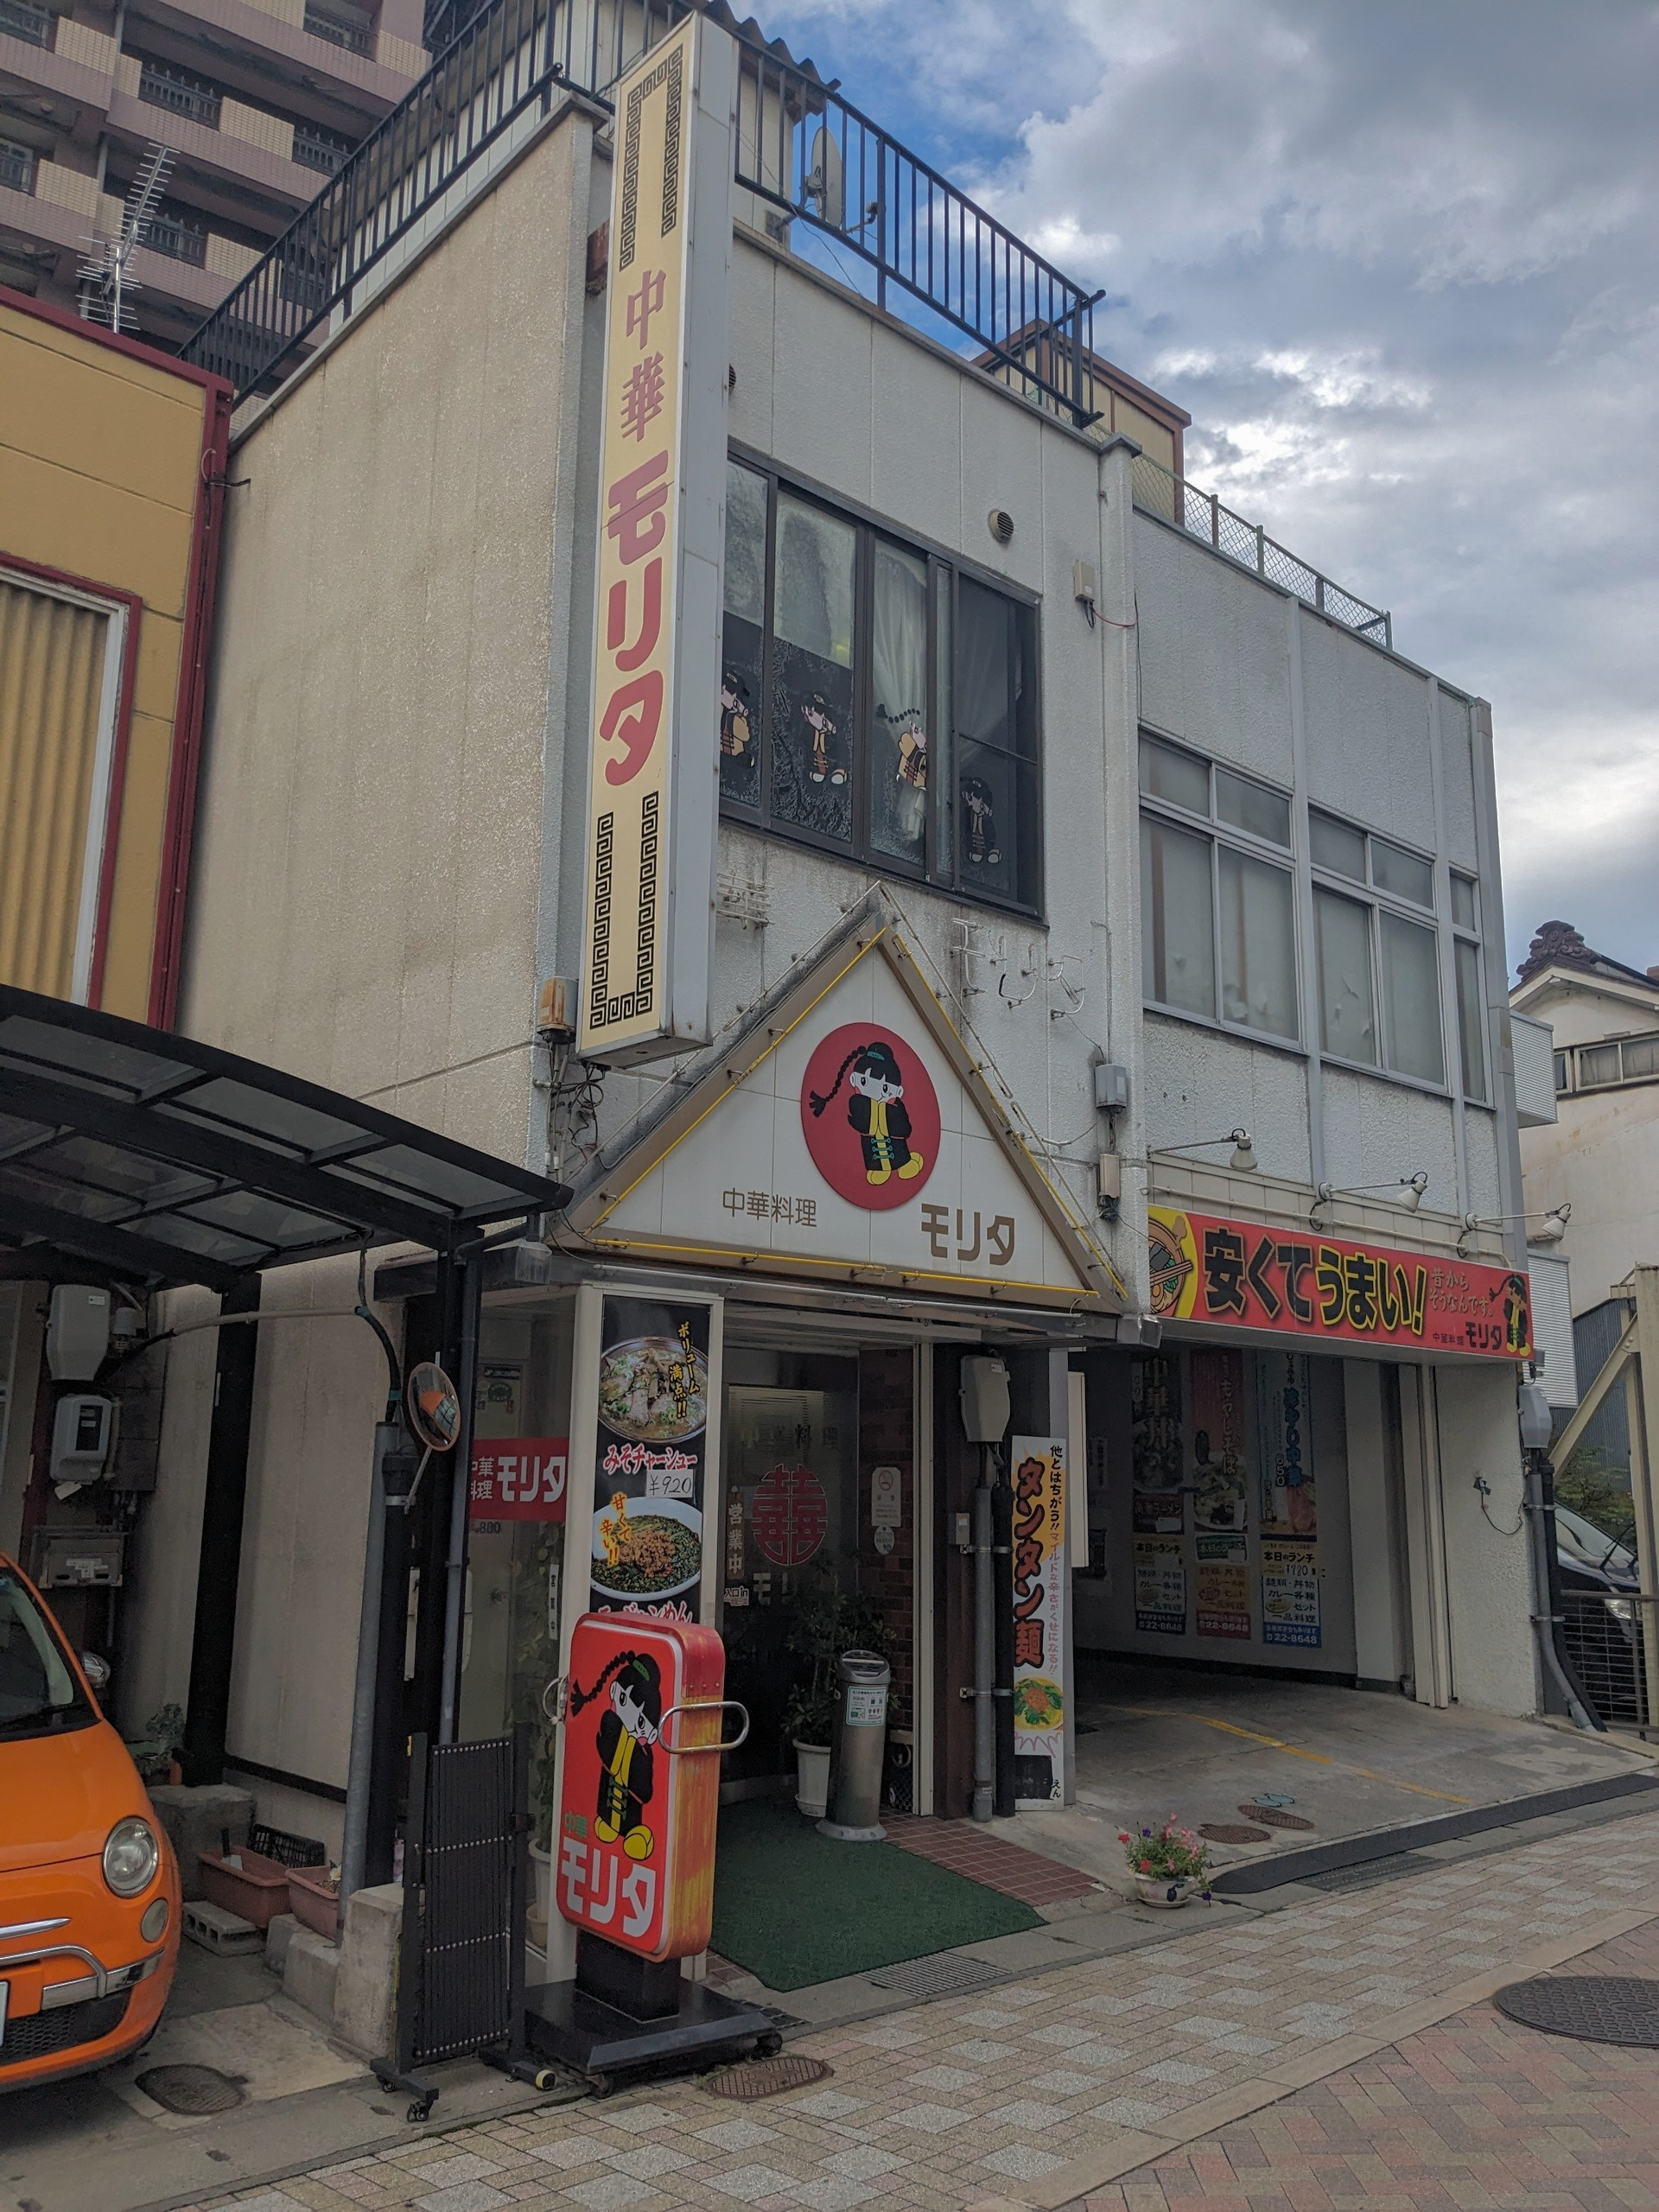
\includegraphics[width=60mm]{C:/Users/user/Documents/ImageProc/task/img/Morita.jpg}
    \caption{線形濃度変換を行う前の画像}
    \label{Morita}
\end{figure}

図\ref{Morita}の画像は雲の色や建物の色など、少しはっきりとしない部分が多く、コントラストが低くなっていることが予想できる。


\end{document}